\documentclass{report}
\usepackage{amsmath}
\usepackage{amssymb}
\usepackage{chapterbib}
\usepackage{docmute}
\usepackage{hyperref}
\usepackage{graphicx}
\usepackage{float}
\usepackage{listings}
\usepackage{xeCJK}
\setCJKmainfont{STKaiti}
\title{机器学习笔记}
\author{李宇奇}
\date{December 2021}
\begin{document}
\maketitle
\tableofcontents
\documentclass{report}
\usepackage{amsmath}
\usepackage{amssymb}
\usepackage{xeCJK}
\setCJKmainfont{STKaiti}
\begin{document}
\chapter{期望方差}
\section{摘要}
本期我们主要学习高斯分布的一些性质
\section{假设}
现在我们有一堆数据:
$$
X=(x_1, x_2, ..., x_N)^T
$$
$$
x_i \in R^p
$$
首先给出我们的模型:高斯线形模型。\\
这里我们为了简化起见,将 $p$ 设为 $1$, 因此 
$$
x \backsim N(\mu, \sigma^2)
$$
$$
\theta=(\mu, \sigma)
$$ 
接下来我们根据这堆数据,通过极大似然估计( MLE )得出其期望与方差\\
下面我们给出似然函数:
$$
\begin{aligned}
p(X|\theta)&=log(\prod_{i=1}^N \frac{1}{\sqrt{2\pi}\sigma} \exp(-\frac{(x_i-\mu)^2}{2\sigma^2})) \\
&=\sum_{i=1}^N log(\frac{1}{\sqrt{2\pi}\sigma} \exp(-\frac{(x_i-\mu)^2}{2\sigma^2}))\\
&=\sum_{i=1}^N log(\frac{1}{\sqrt{2\pi}}) - log(\sigma) - \frac{(x_i-\mu)^2}{2\sigma^2}
\end{aligned}
$$
\section{期望}
下面我们首先使用极大似然估计得出期望 $\mu$ 的估计值
$$
\begin{aligned}
\mu_{MLE}
&=argmax(p(X|\theta))\\
&=argmin(\sum_{i=1}^N (x_i-\mu)^2)
\end{aligned}
$$
对式子求导得到:
$$
\sum_{i=1}^N 2(x_i-\mu)=0
$$
$$
\sum_{i=1}^N x_i - N \mu=0
$$
$$
\mu_{MLE}=\frac{1}{N} \sum_{i=1}^N x_i
$$
\section{方差}
同样的,我们使用极大似然估计得出方差 $\sigma$ 的估计值
$$
\begin{aligned}
\sigma_{MLE}
&=argmax(p(X|\theta))\\
&=argmin(\sum_{i=1}^N log(\sigma)+\frac{(x_i-\mu)^2}{2\sigma^2})
\end{aligned}
$$
同样的,我们对式子求导得到:
$$
\sum_{i=1}^N[\frac{1}{\sigma}-\frac{(x_i-\mu)^2}{\sigma^3}]=0
$$
最后,我们得到估计值:
$$
\sigma_{MLE}^2 = \Sigma_{MLE} = \frac{1}{N} \sum_{i=1}^N (x_i-\mu)^2
$$
\section{偏置估计}
要验证一个估计值是有偏估计还是无偏估计,我们只需计算该估计值的期望即可。
\subsection{$\mu$}
$$
\begin{aligned}
E[\mu_{MLE}]
&=E[\frac{1}{N}\sum_{i=1}^N x_i]\\
&=\frac{1}{N}\sum_{i=1}^N E[x_i]\\
&=\mu
\end{aligned}
$$
因此 $\mu_{MLE}$ 为无偏估计
\subsection{$\sigma$}
首先我们对 $\sigma$ 的估计值进行变形
$$
\begin{aligned}
\sigma_{MLE}^2
&=\frac{1}{N} \sum_{i=1} ^N (x_i - \mu_{MLE})^2\\
&=\frac{1}{N} \sum_{i=1} ^N (x_i^2 - 2x_i\mu_{MLE} + \mu_{MLE}^2)\\
&=\frac{1}{N} \sum_{i=1}^N x_i^2 - 2(\frac{1}{N} \sum_{i=1} ^N x_i) \mu_{MLE} + \mu_{MLE}^2\\
&=\frac{1}{N} \sum_{i=1}^N x_i^2 - 2\mu_{MLE}^2 + \mu_{MLE}^2\\
&=\frac{1}{N} \sum_{i=1}^N x_i^2 - \mu_{MLE}^2\\
&=(\frac{1}{N} \sum_{i=1}^N x_i^2-\mu^2) - (\mu_{MLE}^2-\mu^2)\\
\end{aligned}
$$
令 $f_1=(\frac{1}{N} \sum_{i=1}^N x_i^2-\mu^2)$ , $f_2=(\mu_{MLE}^2-\mu^2)$\\
所以:
$$
\begin{aligned}
E[f_1]
&=E[\frac{1}{N} \sum_{i=1}^N x_i^2 - \mu^2]\\
&=E[\frac{1}{N} \sum_{i=1}^N (x_i^2 - \mu^2)]\\
&=\frac{1}{N} \sum_{i=1}^N E[x_i^2] - E[\mu^2]\\
&=\frac{1}{N} \sum_{i=1}^N E[x_i^2] - \mu^2\\
&=\frac{1}{N} \sum_{i=1}^N E[x_i^2] - (E[x_i])^2\\
&=\sigma^2
\end{aligned}
$$
类似的:
$$
\begin{aligned}
E[f_2]
&=E[\mu_{MLE}^2 - \mu^2]\\
&=E[\mu_{MLE}^2 - (E[\mu_{MLE}])^2]\\
&=Var[\mu_{MLE}]\\
&=Var[\frac{1}{N} \sum_{i=1} ^N x_i]\\
&=\frac{1}{N^2} \sum_{i=1} ^N Var[x_i]\\
&=\frac{1}{N} \sigma^2
\end{aligned}
$$
最后,将 $f_1$ 与 $f_2$ 相加,得到:
$$
E[\sigma_{MLE}^2]=\frac{N-1}{N} \sigma^2
$$
因此我们通过极大似然估计得到的 $\sigma$ 的估计值比真实值略小,所以为有偏估计
而 $\sigma^2$ 的无偏估计为 $\frac{1}{N-1}\sum_{i=1}^N (x_i-\mu_{MLE})^2$

\end{document}
\documentclass{report}
\usepackage{amsmath}
\usepackage{amssymb}
\usepackage{xeCJK}
\setCJKmainfont{STKaiti}
\begin{document}
\chapter{概率视角}
\section{摘要}
本期我们将从概率视角观察多元高斯分布。
\section{先验知识}
$$
x \backsim N(\mu, \sigma^2)
$$
$$
\mu \in R^p, \sigma \in R^p
$$
$$
x_i \backsim N(\mu_i, \sigma_i)
$$
$$
p(x_i) = \frac{1}{\sqrt{2\pi}\sigma_i} \exp(-\frac{(x_i - \mu_i)^2}{2\sigma_i^2})
$$
\section{推导}
首先我们假设每个 $x_i$ 之间是 $iid (independent\ identically\ distribution)$ 独立同分布的。\\
即:
$$
\begin{aligned}
p(x)
&=\prod_{i=1}^p p(x_i)\\
&=\frac{1}{(2\pi)^{\frac{p}{2}}\prod_{i=1}^p \sigma_i} \exp(-\frac{1}{2}\sum_{i=1}^p (\frac{(x_i-\mu_i)^2}{\sigma_i^2}))\\
&=\frac{1}{(2\pi)^{\frac{p}{2}}|\Sigma|^{\frac{1}{2}}} \exp[-\frac{1}{2}
\left (
\begin{matrix}
x_1-\mu_1 & x_2-\mu_2 & ... & x_p - \mu_p
\end{matrix}
\right )
\left (
\begin{matrix}
\frac{1}{\sigma_1^2} & 0 & ... & 0 \\
... & ... & ... & ... \\
0 & ... & 0 & \frac{1}{\sigma_p^2}
\end{matrix}
\right )
\left (
\begin{matrix}
x_1-\mu_1\\
.&\\
.&\\
x_p-\mu_p\\
\end{matrix}
\right )]\\
&=\frac{1}{(2\pi)^{\frac{p}{2}}|\Sigma|^{\frac{1}{2}}} \exp[-\frac{1}{2}(x-\mu)^T \Sigma^{-1}(x-\mu)]
\end{aligned}
$$
以上为多元高斯分布的概率密度函数。\\\\
而我们知道 $\Sigma$ 为半正定矩阵,因此可以进行奇艺值分解。所以我们有:
$$
\begin{aligned}
\Sigma
&=UVU^T\\
&=
\left ( \begin{matrix}
u_1 & ... & u_p
\end{matrix} \right )
\left ( \begin{matrix}
\lambda_1 & 0 & ... & 0\\
... & 0 & ... & ...\\
0 & ... & ... & \lambda_p
\end{matrix} \right )
\left ( \begin{matrix}
u_1^T \\
.\\
.\\
u_p^T
\end{matrix} \right )\\
&=
\left ( \begin{matrix}
u_1\lambda_1 & ... & u_p \lambda_p\\
\end{matrix} \right )
\left ( \begin{matrix}
u_1^T\\
.\\
.\\
u_p^T
\end{matrix} \right )\\
&=\sum_{i=1}^p u_i\lambda_i u_i^T
\end{aligned}
$$
因此
$$
\begin{aligned}
\Sigma^{-1}
&=(UVU^T)^{-1}\\
&=(U^T)^{-1}V^{-1}U^{-1}\\
&=UV^{-1}U^T\\
&=\sum_{i=1}^p u_i \frac{1}{\lambda_i} u_i^T
\end{aligned}
$$
下面我们令 $\Delta = (x-\mu)^T \Sigma^{-1} (x-\mu)$\\
将上面推导的结果代入:
$$
\begin{aligned}
\Delta
&=(x-\mu)^T \Sigma^{-1} (x-\mu)\\
&=(x-\mu)^T \sum_{i=1}^p u_i \frac{1}{\lambda_i}u_i^T (x-\mu)\\
&=\sum_{i=1}^p(x-\mu)^T u_i \frac{1}{\lambda_i}u_i^T (x-\mu)
\end{aligned}
$$
下面我们令 $y_i=(x-\mu)^T u_i$\\
这里 $y_i$ 代表 $x$ 经过中心化后投影到新的正交基 $u_i$ 的坐标值。\\
所以:
$$
\Delta=\sum_{i=1}^p \frac{y_i^2}{\lambda_i}
$$
下面我们再看多元高斯分布的概率密度函数:
$$
p(x)=\frac{1}{(2\pi)^{\frac{p}{2}}|\Sigma|^{\frac{1}{2}}} \exp[-\frac{1}{2}(x-\mu)^T \Sigma^{-1}(x-\mu)]
$$
可以看到式子里与变量 $x$ 相关的只有指数。前面的系数是为了使概率和为 $1$。\\
因此高斯分布的概率与 $\Delta$ 的值直接相关。\\
我们假设 $p=2$ ,即:
$$
\frac{y_1^2}{\lambda_1}+\frac{y_2^2}{\lambda_2}=\Delta
$$
我们惊喜地发现,这与椭圆方程很像。而 $\Delta$ 的值是不固定的,因此对于不同的 $x$ ,这些样本点于平面内形成了一个个同心的椭圆。而这就是高斯分布的性质之一。
\end{document}
\documentclass{report}
\usepackage{amsmath}
\usepackage{amssymb}
\usepackage{xeCJK}
\setCJKmainfont{STKaiti}
\begin{document}
\chapter{边缘概率和条件概率}
\section{摘要}
本节我们学习多元高斯分布的边缘概率和条件概率
\section{先验知识}
在上一节中,我们推导了多元高斯分布的概率密度函数:
$$
x \backsim N(\mu, \Sigma) = \frac{1}{(2\pi)^{\frac{p}{2}}|\Sigma|^\frac{1}{2}}\exp(-\frac{1}{2}(x-\mu)^T \Sigma^{-1}(x-\mu))
$$
现在我们将随机变量 $x$ 拆分为两部分:
$$
x \in R^p \quad x_a \in R^m \quad x_b \in R^n \quad m+n=p \quad 
$$
$$
x = 
\left (
\begin{matrix}
x_a \\
x_b \\
\end{matrix}
\right )
\quad 
\mu = 
\left (
\begin{matrix}
\mu_a \\
\mu_b \\
\end{matrix}
\right ) \quad
\Sigma=
\left (
\begin{matrix}
\Sigma_{aa} & \Sigma_{ab}\\
\Sigma_{ba} & \Sigma_{bb}\\
\end{matrix}
\right )
$$
\section{定理}
$$
X \backsim N(\mu, \Sigma) \quad Y=AX+B  \Longrightarrow Y \backsim N(A\mu+B, A \Sigma A^T)
$$
\section{推导边缘概率}
$$
x_a = \left (\begin{matrix}I & 0\end{matrix}\right )\left (\begin{matrix}x_a \\x_b\\\end{matrix}\right ) + 0
$$
$$
E[x_a] = \left (\begin{matrix}I & 0\end{matrix}\right )\left (\begin{matrix}\mu_a \\\mu_b \\\end{matrix}\right ) = \mu_a
$$
$$
\begin{aligned}Var[x_a] &= \left (\begin{matrix}I & 0\end{matrix}\right )\left (\begin{matrix}\Sigma_{aa} & \Sigma_{ab} \\\Sigma_{ba} & \Sigma_{bb} \\\end{matrix}\right )\left (\begin{matrix}I \\0\end{matrix}\right ) \\&= \left (\begin{matrix}\Sigma_{aa} & \Sigma_{ab} \end{matrix}\right )\left (\begin{matrix}I \\0\end{matrix}\right )\\&=\Sigma_{aa}\end{aligned}
$$
$$
\therefore x_a \backsim N(\mu_a, \Sigma_{aa})
$$
\section{推导条件概率}
我们设:
$$
\begin{cases}
x_{b.a}=x_b - \Sigma_{ba} \Sigma_{aa}^{-1} x_a \\
\mu_{b.a} = \mu_b - \Sigma_{b.a} \Sigma_{aa}^{-1} \mu_a \\
\Sigma_{bb.a}=\Sigma_{bb} - \Sigma_{ba} \Sigma_{aa}^{-1} \Sigma_{ab}
\end{cases}
$$
$$
\begin{aligned}
x_{b.a} &= x_b - \Sigma_{ba} \Sigma_{bb}^{-1} x_a \\
&=
\left (
\begin{matrix}
- \Sigma_{ba} \Sigma_{bb}^{-1} & I\\
\end{matrix}
\right )
\left (
\begin{matrix}
x_a \\
x_b \\
\end{matrix}
\right ) + 0
\end{aligned}
$$
$$
\begin{aligned}
E[x_{b.a}]
&=
\left (
\begin{matrix}
-\Sigma_{ba} \Sigma_{aa}^{-1} & I
\end{matrix}
\right )
\left (
\begin{matrix}
\mu_a \\
\mu_b \\
\end{matrix}
\right )\\
&=\mu_b - \Sigma_{ba} \Sigma_{aa}^{-1} \mu_a\\
&=\mu_{b.a}
\end{aligned}
$$
$$
\begin{aligned}
Var[x_{b.a}]
&= \left ( \begin{matrix}
-\Sigma_{ba} \Sigma_{aa}^{-1} & I
\end{matrix} \right )
\left ( \begin{matrix}
\Sigma_{aa} & \Sigma_{ab} \\
\Sigma_{ba} & \Sigma_{bb} \\
\end{matrix} \right )
\left ( \begin{matrix}
-\Sigma_{aa}^{-1} \Sigma_{ba}^T \\
I
\end{matrix} \right ) \\
&=\left ( \begin{matrix}
0 & \Sigma_{bb} - \Sigma_{ba} \Sigma_{aa}^{-1} \Sigma_{ab} \\
\end{matrix} \right ) 
\left ( \begin{matrix}
-\Sigma_{aa}^{-1} \Sigma_{ba}^T \\backsim
I
\end{matrix} \right ) \\
&=\Sigma_{bb} - \Sigma_{ba} \Sigma_{aa}^{-1} \Sigma_{ab}\\
&=\Sigma_{bb.a}
\end{aligned}
$$
$$
\therefore x_{b.a} \backsim N(\mu_{b.a}, \Sigma_{bb.a})
$$
$$
\begin{cases}
\mu_{b.a} = \mu_b - \Sigma_{ba} \Sigma_{aa}^{-1} \mu_a \\
\Sigma_{bb.a}=\Sigma_{bb} - \Sigma_{ba} \Sigma_{aa}^{-1} \Sigma_{ab}
\end{cases}
$$
我们将式子稍作变形:
$$
\begin{aligned}
x_{b.a}
&=x_b - \Sigma_{ba} \Sigma_{aa}^{-1} x_a\\
x_b | x_a&=x_{b.a} + \Sigma_{ba} \Sigma_{aa}^{-1} x_a\\
&=I x_{b.a} + C\\
\end{aligned}
$$
此处,协方差矩阵的部分 $\Sigma_{ba} \ \Sigma_{aa}$ 都是可以通过计算得到的,因此可以视为常数。\\
而我们此处要求的是 $x_b | x_a$ ,因此 $x_a$ 也是已知的,因此上式的第二项可以视为常数。\\\\
因此:
$$
E[x_b|x_a]=I E[x_{b.a}] + C = \mu_{b.a} + \Sigma_{ba} \Sigma_{aa}^{-1} x_a
$$
$$
Var[x_b|x_a]=IVar[x_{b.a}]I^T=\Sigma_{bb.a}
$$
因此我们得出了高斯分布的条件概率:
$$
x_b|x_a \backsim N(\mu_{b.a} + \Sigma_{ba} \Sigma_{aa}^{-1} x_a, \Sigma_{bb.a})
$$
\end{document}
\documentclass{report}
\usepackage{amsmath}
\usepackage{amssymb}
\usepackage{xeCJK}
\setCJKmainfont{STKaiti}
\begin{document}
\chapter{联合分布}
\section{摘要}
本节我们学习高斯联合分布。
\section{已知}
$$
x \sim N(x|\mu, \Lambda^{-1})
$$
$$
y|x \sim N(y|Ax+b, L^{-1})
$$
\section{隐含条件}
$$
y = Ax+b+\epsilon, \quad \epsilon \sim N(0, L^{-1}), \quad x \perp \epsilon
$$
\section{所求}
$$
\begin{cases}
p(y)\\
\\
p(x|y)
\end{cases}
$$
\section{推导}
\subsection{推导 $p(y)$}
$$
E[y] = A E[x] + b + E[\epsilon]=A \mu + b
$$
$$
Var[y] = A \Lambda^{-1} A^T
$$
$$
\therefore y \sim N(A\mu +b, A\Lambda^{-1} A^T)
$$
\subsection{推导 $p(x|y)$}
\subsubsection{构造分布 $z$}
此处我们构造一个分布:
$$
z = 
\left (
\begin{matrix}
x\\
y\\
\end{matrix}
\right )
\sim N(
\left [
\begin{matrix}
\mu\\
A\mu+b\\
\end{matrix}
\right ],
\left [
\begin{matrix}
\Lambda^{-1}&\Delta\\
\Delta&A\Lambda^{-1} A^T\\
\end{matrix}
\right ]
)
$$
$$
\begin{aligned}
\Delta
&=cov(x,y)\\
&=E[(x-E[x])(y-E[y])^T]\\
&=E[(x-\mu)(y-A\mu - b)^T]\\
&=E[(x-\mu)(Ax+b+ \epsilon -A\mu -b)^T)]\\
&=E[(x-\mu)(Ax-A\mu + \epsilon)^T]\\
&=E[(x-\mu)(x-\mu)^T A^T + (x-\mu)\epsilon^T]\\
&=E[(x-\mu)(x-\mu)^T]A^T + E[(x-\mu)\epsilon^T] \\
\because &x \perp \epsilon\\
\therefore &=E[(x-\mu)(x-\mu)^T]A^T\\
&=\Lambda^{-1}A^T
\end{aligned}
$$
$$
\therefore z=
\left ( \begin{matrix}
x\\y
\end{matrix} \right )
\sim N(
\left [
\begin{matrix}
\mu\\
A\mu+b\\
\end{matrix}
\right ],
\left [
\begin{matrix}
\Lambda^{-1}&\Lambda^{-1}A^T\\
\Lambda^{-1}A^T&A\Lambda^{-1} A^T\\
\end{matrix}
\right ]
)
$$
\subsubsection{构造分布 $x.y$}
我们设:
$$
\begin{aligned}
x.y 
&= x - \Sigma_{xy} \Sigma_{yy}^{-1}y\\
&= x - (\Lambda^{-1} A^T)(A \Lambda^{-1}A^T)^{-1}y\\
&= x - A^{-1}y\\
&= 
\left ( \begin{matrix}
I& -A^{-1}
\end{matrix} \right )
\left ( \begin{matrix}
x\\
y
\end{matrix} \right )
\end{aligned}
$$
$$
\begin{aligned}
E[x.y] 
&= E[x] - A^{-1} E[y]\\
&= \mu - A^{-1}(A\mu+b)\\
&= -A^{-1}b
\end{aligned}
$$
$$
\begin{aligned}
Var[x.y]
&= 
\left ( \begin{matrix}
I& -A^{-1}
\end{matrix} \right )
Var[z]
\left ( \begin{matrix}
I\\
-(A^{-1})^T\\
\end{matrix} \right )\\
&= 
\left ( \begin{matrix}
I& -A^{-1}
\end{matrix} \right )
\left (
\begin{matrix}
\Lambda^{-1}&\Lambda^{-1}A^T\\
\Lambda^{-1}A^T&A\Lambda^{-1} A^T\\
\end{matrix}
\right )
\left ( \begin{matrix}
I\\
-(A^{-1})^T\\
\end{matrix} \right )\\
&=
\left ( \begin{matrix}
\Lambda^{-1}-A^{-1} \Lambda^{-1}A^T & 0
\end{matrix} \right )
\left ( \begin{matrix}
I\\
-(A^{-1})^T\\
\end{matrix} \right )\\
&=\Lambda^{-1}-A^{-1} \Lambda^{-1}A^T
\end{aligned}
$$
$$
\therefore x.y \sim N(-A^{-1}b, \Lambda^{-1}-A^{-1} \Lambda^{-1}A^T)
$$
\subsubsection{构造分布 $x|y$}
我们有:
$$
x|y = x.y + A^{-1}y
$$
这里,我们可以将 $A^{-1}y$ 视为常数 $C$.\\
那么:
$$
x|y = x.y + C
$$
$$
E[x|y] = A^{-1}y - A^{-1}b
$$
$$
Var[x|y]= Var[x.y]
$$
$$
\therefore x|y \sim N(A^{-1}y - A^{-1}b, \Lambda^{-1}-A^{-1} \Lambda^{-1}A^T)
$$
现在,我们根据一个边缘分布和条件分布,通过构造联合分布,求出了另一个边缘分布和条件分布。
\end{document}
\documentclass{report}
\usepackage{amsmath}
\usepackage{amssymb}
\usepackage{xeCJK}
\usepackage{hyperref}
\usepackage{graphicx}
\usepackage{listings}
\setCJKmainfont{STKaiti}
\begin{document}
\chapter{线性回归}
\section{摘要}
你好,我是生而为弟。\\
在学习NLP的过程中,我对于公式的推导完全不会,因此我决定从头学习机器学习的理论推导。\\
本期主要分为两个部分:
\begin{itemize}
	\item[] 第一部分将从矩阵,几何,概率三个视角,对线性回归-最小二乘法的闭式解进行推导,并提供参考代码。
	\item[] 第二部分将从矩阵和概率两个视角,对带正则化的最小二乘法的闭式解进行推导,并构造一个完整的线性回归类,同时实现闭式解求法与梯度下降解法。
\end{itemize}
\section{介绍}
线性回归模型是利用线性函数对一个或多个自变量和因变量($y$)之间关系进行拟合的模型。\\
目标变量($y$)为连续数值型 ,如:房价,人数,降雨量 回归模型是寻找一个输入变量到输出变量之间的映射函数。\\
回归问题的学习等价于函数拟合:使用一条函数曲线使其很好的拟合已知数据且能够预测未知数据。\\
回归问题分为模型的学习和预测两个过程。基于给定的训练数据集构建一个模型,根据新的输入数据预测相应的输出。
\section{不带正则化的算法}
\subsection{矩阵视角}
注:一般情况下,我们讨论的向量都是列向量,因此推导过程中为保证矩阵的形状,会大量使用转置符\\
已知数据集$D=\{(x_1,y_1),(x_2,y_2)...(x_n,y_n)\}$\\
其中$x_i\in R^p,y_i\in R,i=1,2,...,n$\\
$$
X=(x_1,x_2,...,x_n)^T=\begin{pmatrix}
x_{11}&x_{12}&...&X_{1p}\\
x_{21}&x_{22}&...&x_{2p}\\
.&.&.&.&\\
.&.&.&.&\\
.&.&.&.&\\
x_{n1}&x_{n2}&...&x_{np}\\
\end{pmatrix}_{np}
$$
$$
Y=(y1,y2,...,y_n)_{n1}^T
$$
这是我们建立的模型:$f(w)=w^Tx+w_0x_0。$\\
一般令$x_0=1$,而$b=w_0x_0$,$b$是偏置(bias),$w$为权重(weight),下面为了推导的方便,我们将$w_0$并入$w$中,$x_0$并入$X$中\\
因此模型更为$f(w)=w^Tx$
最小二乘法的损失函数为:
$$
L(w)=\sum_{i=1}^{i=n}\|y_i-w^T x_i\|_2^2
$$
$$
=\begin{pmatrix}
y_1-w^Tx_1&y_2-w^Tx_2&...&y_n-w^Tx_n
\end{pmatrix}
\begin{pmatrix}
y_1-w^Tx_1\\
y_2-w^Tx_2\\
.\\
.\\
.\\
y_n-w^Tx_n\\
\end{pmatrix}
$$
$$
=(Y^T-w^TX^T)(Y^T-w^TX^T)^T
$$
$$
=(Y^T-w^TX^T)(Y-Xw)
$$
$$
=Y^TY-w^TX^TY-Y^TXw+w^TX^TXw
$$
仔细观察发现第二三项是互相转置的,而观察它的矩阵形状: $(1,p)(p,n)(n,1)=(1,1)$\\
得知这两项为标量,而标量的转置还是本身,因此可将两项合并,得
$$
L(w)=Y^TY-2w^TX^TY+w^TX^TXw
$$
因此$\hat{w}=argmin(L(w))$
下面要求出$L(w)$的最小值,对$L(w)$求导\\
可以看到式子共三项,第一项与$w$无关,可以去掉。那么剩余两项就要涉及到矩阵求导了\\
关于矩阵求导,笔者推荐一位博主的三篇文章(比教科书还详细,严谨,每个公式都有证明)
\begin{itemize}
	\item \href{https://zhuanlan.zhihu.com/p/263777564}{矩阵求导——本质篇}
	\item \href{https://zhuanlan.zhihu.com/p/273729929}{矩阵求导——基础篇}
	\item \href{https://zhuanlan.zhihu.com/p/288541909}{矩阵求导——进阶篇}
\end{itemize}
下面为上述两项的导数求解过程:\\
因为$X,Y$为常数矩阵,因此可直接求出导数,但因为是对$w$求导,因此要对结果进行转置
$$
\frac{d(2w^TX^TY)}{dw}=2X^TY
$$
下面求解第三项
$$
d(w^TX^TXw)=tr(d(w^TX^TXw))=tr(X^TXd(w^Tw))
$$
$$
=tr(X^TX(d(w^T)w+w^Td(w)))=tr(X^TXw(dw)^T)+tr(X^TXw^Tdw)
$$
$$
=tr(w^TX^TXdw)+tr(X^TXw^Tdw)=tr(2X^TXw^Tdw)
$$
所以
$$
\frac{d(w^TX^TXw)}{dw}=2wX^TX
$$
所以$\frac{dL(w)}{dw}=2X^TXw-2X^TY$\\
令导数等于0,得出最小二乘的闭式解:
$$
\hat{w}=(X^TX)^{-1}X^TY
$$
\subsection{几何视角}
$$
X=(x_1,x_2,...,x_n)^T=\begin{pmatrix}
x_{11}&x_{12}&...&X_{1p}\\
x_{21}&x_{22}&...&x_{2p}\\
.&.&.&.&\\
.&.&.&.&\\
.&.&.&.&\\
x_{n1}&x_{n2}&...&x_{np}\\
\end{pmatrix}_{np}
$$
$$
Y=(y1,y2,...,y_n)_{n1}^T
$$
在几何视角下,我们将$X$看作是一个$p$维的向量\\
$X$的第一维是$(x_{11},x_{21},...,x_{n1})$,$X$的第$p$维是$(x_{1p},x_{2p},...,x_{np})$
而这里的$Y$被看作是一个一维的向量\\
现在我们假设$p=2$,因为比较好画。示意图如下(俺真的画了好久,观众老爷们给波三连吧)\\\\
\begin{figure}
\center
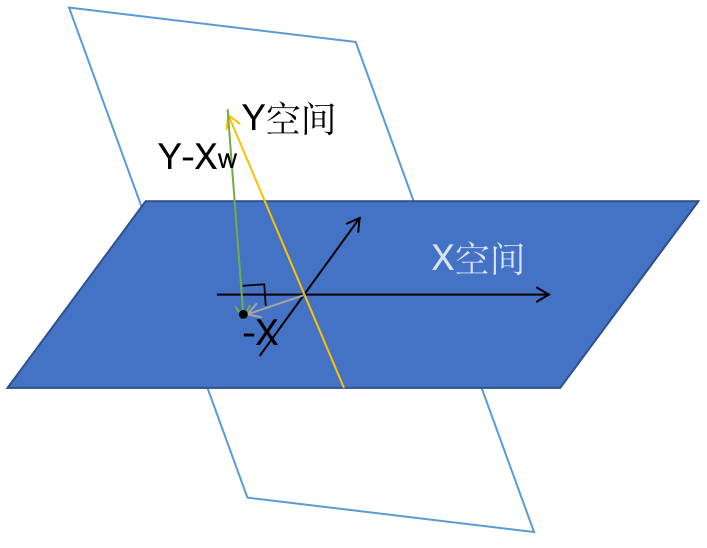
\includegraphics[width = 0.7 \textwidth]{/Users/btobab/TeX-Projects/figures/1}
\end{figure}
将模型改为$f(w)=Xw$,意为对$X$向量施以$w$权重的放缩\\
而最小二乘的几何意义就是找到一个$w$,使得$Y-Xw$这个向量到$X$空间的距离最小,那最小的情况当然就是与$X$空间垂直\\
所以我们有式子$X^T(Y-Xw)=0$\\
从而求解$w$:
$$
X^TXw=X^TY
$$
$$
\hat{w}=(X^TX)^{-1}X^TY
$$
可以看到求出的$w$与矩阵视角的结果相同。
\subsection{概率视角}
首先明确,现实中是很难用一条直线去拟合分布的。真实的数据必然存在一定的随机性,也就是噪声。\\
因此我们假设噪声$\epsilon\backsim N(0,\sigma^2)$\\
所以$y=f(w)+\epsilon=w^Tx+\epsilon$\\
所以$y|x;w\backsim N(w^Tx,\sigma^2)$\\
带入高斯分布的概率密度函数:
$$
p(y|x;w)=\frac{1}{\sqrt{2\pi}\sigma}e^{-\frac{(y-w^Tx)^2}{2\sigma^2}}
$$
下面使用 MLE (极大似然估计):\\
注:所谓极大似然估计,即通过大量的采样得到相对频率,去逼近概率\\
我们设一个函数$\mathcal{L}(w)=\log{p(Y|X;w)}$\\
因为$n$个数据之间是独立的,因此可以将概率改为连乘的形式。\\
$\mathcal{L}(w)=\log{\Pi_{i=1}^np(y_i|x_i;w)}=\Sigma_{i=1}^n \log{p(y_i|x_i;w)}$\\
将高斯分布的概率密度函数带入式子:\\
$\mathcal{L}(w)=\Sigma_{i=1}^n(\log{\frac{1}{\sqrt{2\pi}\sigma}}-\frac{(y-w^Tx)^2}{2\sigma^2})$\\
因为前一项与$w$无关,所以可以忽略\\
所以:
$$
\begin{aligned}
\hat{w}
&=argmax \mathcal{L}(w)\\
&=argmax \Sigma_{i=1}^n -\frac{(y-w^Tx)^2}{2\sigma^2}\\
&=argmin \Sigma_{i=1}^n (y-w^Tx)^2
\end{aligned}
$$
而使用极大似然估计得到的结论正是最小二乘法的定义。\\
这也恰好说明,最小二乘法隐藏着一个噪声为高斯分布的假设。
\section{不带正则项的实作}
\begin{lstlisting}[language={python}]
%matplotlib inline
import numpy as np
import matplotlib.pyplot as plt

# 样本数
n = 1000
# 噪声
epsilon = 1
X = np.expand_dims(np.linspace(0,100,1000), axis=-1)
w = np.asarray([5.2])
Y = X  w
# 增加噪声扰动
X += np.random.normal(scale=epsilon, size=(X.shape))
X_T = X.transpose()
w_hat = np.matmul(np.linalg.pinv((np.matmul(X_T, X))), np.matmul(X_T, Y))
print(w_hat)
plt.scatter(X, Y, s=3, c="y")
Y_hat = X  w_hat
plt.plot(X, Y_hat)
plt.show()
\end{lstlisting}
\section{带正则化的算法}
\subsection{矩阵视角}
首先给出带正则项的新损失函数:
$$
\mathcal{L}(w)=\Sigma_{i=1}^{n}||y_i-w^T  x_i||^2 + \lambda  ||w||^2
$$
然后引用不带正则化的矩阵视角的损失函数的推导形式:
$$
\mathcal{L}(w)=Y^TY-2w^TX^TY+w^TX^TX w+\lambda  ||w||^2
$$
所以$\hat{w}=argmax(\mathcal{L}(w))$\\
对$\mathcal{L}(w)$求导,得到:
$$
\frac{\partial \mathcal{L}(w)}{\partial w}=2X^TXw-2X^T Y+2\lambda  w 
$$
令导数为0,得到带正则化的最小二乘法的闭式解:
$$
\hat{w}=(X^TX+\lambda  I)^{-1} X^TY
$$
$I$为单位矩阵
\subsection{概率视角}
假设噪声$\epsilon \backsim N(0,\sigma_1^2) \ w \backsim N(0,\sigma_2^2)$\\
因为$y=w^T x + \epsilon$\\
所以$y|w \backsim N(w^T x,\sigma_1^2)$
下面我们使用 MAP(最大后验估计):
由贝叶斯定理得:
$$
P(w|Y)=\frac{P(Y|w) P(w)}{P(Y)}
$$
其中$P(w)$为先验概率,$P(Y|w)$为似然概率,$P(Y)$为归一化概率,先验概率乘似然概率并归一化得到后验概率$P(w|Y)$
其中$P(Y)$实际上为常数,因此:
$$
\hat{w}=argmax(P(w|Y))=argmax(P(Y|w) P(w))=argmax(log(P(Y|w) P(w)))
$$
因为每个样本间是独立的,因此可以将概率连乘
$$
=argmax(log(\prod_{i=1}^n P(y_i|w) P(w)))=argmax(\sum_{i=1}^n log(P(y_i|w)+ log(P(w))))
$$
带入高斯分布的概率密度函数,得到:
$$
\hat{w}=argmax(\sum_{i=1}^nlog(\frac{1}{\sqrt{2\pi} \sigma_1})-\frac{(y_i-w^T x_i)^2}{2\sigma_1^2}+log(\frac{1}{\sqrt{2 \pi} \sigma_2})-\frac{w^2}{2\sigma_2^2})
$$
因为$\sigma_1,\sigma_2$都为超参数,因此可以省略\\
所以:
$$
\hat{w}=argmin(\sum_{i=1}^n \frac{(y_i-w^T x_i)^2}{2\sigma_1^2}+\frac{w^2}{2\sigma_2^2})
$$
$$
=argmin(\sum_{i=1}^n (y_i-w^T x_i)^2+\frac{\sigma_1^2}{\sigma_2^2} w^2)
$$
可以看到,使用 MAP 推导出的结果正是带正则项的最小二乘的定义
\newpage
\section{带正则项的实作}
\begin{lstlisting}[language={python}]
import os
os.chdir("../")
import numpy as np
import matplotlib.pyplot as plt
from models.linear_models import LinearRegression

X_ = np.expand_dims(np.linspace(0, 10, 1000), axis=-1)
X = np.c_[X_, np.ones(1000)]
w = np.asarray([5.2, 1])
Y = X.dot(w)
X = np.r_[X, np.asarray([[11, 1], [12, 1], [13, 1]])]
Y = np.r_[Y, np.asarray([100, 110, 120])]

model = LinearRegression(l2_ratio=1e1, epoch_num=1000, lr=1e-2, batch_size=100, if_standard=False)
model.fit(X[:, :-1], Y)
print(model.get_params())
model.draw(X[:, :-1], Y)
\end{lstlisting}
\end{document}
\documentclass{report}
\usepackage{amsmath}
\usepackage{amssymb}
\usepackage{xeCJK}
\usepackage{listings}
\setCJKmainfont{STKaiti}
\begin{document}
\chapter{感知机}
\section{摘要}
众所周知,线性分类分为两种:
\begin{itemize}
	\item 硬输出(直接输出样本的类别):
	\begin{itemize}
	\item 感知机
	\item 线性判别分析
	\end{itemize}
	\item 软输出(输出样本属于某类别的概率):
	\begin{itemize}
	\item 高斯判别分析
	\item 逻辑回归
	\end{itemize}
\end{itemize}
本期将介绍一种简单的线性二分类模型:感知机(Perceptron),它的要求比较松,只要能找到一个超平面将正负样本分割开就行。
\section{算法思想}
\subsection{错误驱动}
从字面上我们就可以看出,感知机模型的思路就是先随机初始化模型的参数,然后根据当前参数是否能够正确分割正负样本,通过错误来更新自己的参数。
\section{算法}
首先给出模型的目标函数:
$$
f(x)=sign(w^Tx)
$$
其中,$sign$是一个符号函数:
$$
sign(a)=
\begin{cases}
+1,\,\,a>0\\
-1,\,\,a\le0\\
\end{cases}
$$
那么根据上面提到的感知机的思想:错误驱动\\
我们很容易写出该模型的损失函数:
$$
L(w)=\sum_{i=1}^n I\{w^Tx_i  y_i<0 \}
$$
其中,$I$是指示函数,表示有哪些元素属于该集合。\\
而判断条件也很好理解。我们注意到:
\begin{itemize}
	\item 当$y_i>0$,即$y_i$为正例;
	\begin{itemize}
	\item 此时,若$w^Tx_i<0$,则说明该样本被错误分类($w^Tx_i y_i<0$)
	\item 若$w^Tx_i>0$,则说明该样本被正确分类($w^Tx_i y_i>0$)
	\end{itemize}
	\item 当$y_i<0$,即$y_i$为负例;
	\begin{itemize}
	\item 此时,若$w^Tx_i<0$,则说明该样本被正确分类($w^Tx_i y_i>0$)
	\item 若$w^Tx_i>0$,则说明该样本被错误分类($w^Tx_i y_i<0$
	\end{itemize}
\end{itemize}
我们最终发现,当$w^Tx_i  y_i<0$时,可以表示样本被模型错误分类。
好,我们现在再回头看损失函数,我们惊奇地发现,这个损失函数居然是不可导的,没法梯度下降了,这可肿么办尼。

因此我们放宽了条件,损失函数更为:
$$
L(w)=\sum_{(x_i,y_i)\in M} -w^Tx_i y_i
$$
$M$表示被错误分类的样本的集合。

在$w^Tx_i y_i$前面加个负号,就可以得到正的损失值了。这样就可以使用梯度下降算法更新参数$w$了。

至于这个损失函数的导数也很容易求嘛:

$$
\frac{dL(w)}{dw}=\sum_{(x_i,y_i)\in M} -x_i y_i
$$
\newpage
\section{实作}
\begin{lstlisting}[language={python}]
import os
os.chdir("../")
import numpy as np
from models.linear_models import Perceptron


model = Perceptron(10000, lr=1e-2)
x = np.linspace(0, 100, num=100)
w1, b1 = 0.1, 5
w2, b2 = 0.2, 10
epsilon = 2
k = 0.15
b = 8
w = np.asarray([-k, 1])
v1 = x * w1 + b1 + np.random.normal(scale=epsilon, size=x.shape)
v2 = x * w2 + b2 + np.random.normal(scale=epsilon, size=x.shape)
x1 = np.c_[x, v1]
x2 = np.c_[x, v2]
x = np.r_[x1, x2]
y = np.sign(x.dot(w) - b)
model.fit(x, y)
model.draw(x)
\end{lstlisting}
\end{document}
\documentclass{report}
\usepackage{amsmath}
\usepackage{amssymb}
\usepackage{xeCJK}
\usepackage{listings}
\setCJKmainfont{STKaiti}
\begin{document}
\chapter{线性判别分析}
\section{摘要}
本期我们将学习二分类-硬输出的另一种算法:线性判别分析,这实际上也是一种降维的算法。\\
选定一个方向,将高维样本投影到这个方向上,从而对样本进行二分类。
\section{算法思想}
线性判别分析的核心思想是使投影后的数据满足两个条件:
\begin{itemize}
	\item 相同类内部的样本距离接近
	\item 不同类别之间的距离较大
\end{itemize}
\section{算法}
要降维,我们首先要知道如何计算投影。\\\\
我们假定样本为$x$,沿$w$方向做投影\\
我们知道:$w x=||w||\ ||x|| \cos{\theta}$\\
这里我们假设 $||w||=1$,确定唯一的 $w$,防止放缩导致无数解\\
所以 $w\ x=||x||\cos{\theta}$\\
而 $||x||\cos{\theta}$ 正是投影的定义\\
所以样本点在向量 $w$ 上的投影长度为 $w\ x$\\
故投影长度 $z=w^T\ x$\\
我们假定属于两个类的样本数量分别为 $N1,N2$\\
下面对于第一个条件:相同类内部的样本距离接近,我们使用方差矩阵来表征每个类内部的总体分布。这里我们使用协方差矩阵的定义,用$S$表示原数据$x$的协方差矩阵
\begin{equation}
\begin{aligned}C_1: Var_z[C_1]&=\frac{1}{N_1}\sum_{i=1}^{N_1} (z_i-\bar{z_{c1}})(z_i-\bar{z_{c1}})^T\\
&=\frac{1}{N_1}\sum_{i=1}^{N_1}(w^T x_i-\frac{1}{N_1}\sum_{j=1}^{N_1}w^T x_j)(w^T x_i-\frac{1}{N_1}\sum_{j=1}^{N_1}w^T x_j)^T \\&=w^T \frac{1}{N_1}\sum_{i=1}^{N_1}(x_i-\frac{1}{N_1}\sum_{j=1}^{N_1} x_j)(x_i-\frac{1}{N_1}\sum_{j=1}^{N_1} x_j)^T w\\&=w^{T} \frac{1}{N_{1}} \sum_{i=1}^{N_{1}}\left(x_{i}-\bar{x_{c 1}}\right)\left(x_{i}-\bar{x_{c 1}}\right)^{T} w\\&=w^T S_1 w\\C_2: Var_z[C_2]&=\frac{1}{N_2}\sum_{i=1}^{N_2} (z_i-\bar{z_{c2}})(z_i-\bar{z_{c2}})^T\\&=w^T S_2 w
\end{aligned}
\end{equation}
所以类内距离可以记为:
$$
Var_z[C_1]+Var_z[C_2]=w^T(S_1+S_2)w
$$
对于第二个条件:不同类别之间的距离较大\\
我们可以用两个类的投影均值表示类间距离:
\begin{equation}
\begin{aligned}
(z_{c1}-z_{c2})^2&=(\frac{1}{N_1}\sum_{i=1}^{N_1}w^T x_i - \frac{1}{N_2}\sum_{i=1}^{N_2}w^T x_i)^2\\
&=(w^T(\frac{1}{N_1}\sum_{i=1}^{N_1} x_i - \frac{1}{N_2}\sum_{i=1}^{N_2} x_i))^2\\
&=(w^T(\bar{x_{c1}}-\bar{x_{c2}}))^2\\
&=w^T(\bar{x_{c1}}-\bar{x_{c2}})(\bar{x_{c1}}-\bar{x_{c2}})^T w
\end{aligned}
\end{equation}
好,现在再回头看看我们的两个条件:
\begin{itemize}
	\item 相同类内部的样本距离接近
	\item 不同类别之间的距离较大
\end{itemize}
我们很容易给出一个直观的损失函数:
$$
L(w)=\frac{Var_z[C_1]+Var_z[C_2]}{(z_{c1}-z_{c2})^2}
$$
通过最小化损失函数,我们得到最优的$w$:
\begin{equation}
\begin{aligned}
\hat{w}=argmin(L(w))&=argmin(\frac{Var_z[C_1]+Var_z[C_2]}{(z_{c1}-z_{c2})^2})\\
&=argmin(\frac{w^T(S_1+S_2)w}{w^T(\bar{x_{c1}}-\bar{x_{c2}})(\bar{x_{c1}}-\bar{x_{c2}})^T w})\\
&=argmin(\frac{w^T S_w w}{w^T S_b w})
\end{aligned}
\end{equation}
其中:
\begin{itemize}
	\item $S_w$ 为with-class: 类内方差
	\item $S_b$ 为between-class: 类间方差
\end{itemize}
下面对上式做偏导:
$$
\begin{aligned}
\frac{\partial{L(w)}}{\partial{w}}&=\frac{\partial}{\partial{w}}(w^T S_w w)(w^T S_b w)^{-1}\\
&=2 S_{b} w\left(w^{T} S_{w} w\right)^{-1}-2 w^{T} S_{b} w\left(w^{T} S_{w} w\right)^{-2} S_{w} w=0\\
\end{aligned}
$$
对方程做变换:
$$
\begin{aligned}
\left(w^{T} S_{b} w\right) S_{w} w&=S_{b} w\left(w^{T} S_{w} w\right)\\
\left(w^{T} S_{b} w\right) w&=S_{w}^{-1}S_{b} w\left(w^{T} S_{w} w\right)
\end{aligned}
$$
注意到,$w^T S_b w$与$w^T S_w w$的形状为: $(1,p) (p,p) (p,1)=(1,1)$\\
因此这两项都为标量,只是对向量的大小进行放缩,不改变方向,因此上式更为:
$$
w \propto S_{w}^{-1} S_{b} w=S_{w}^{-1}\left(\bar{x_{c 1}}-\bar{x_{c 2}}\right)\left(\bar{x_{c 1}}-\bar{x_{c 2}}\right)^{T} w 
$$
又因为$\left(\bar{x_{c 1}}-\bar{x_{c 2}}\right)^{T} w$也为标量,因此得到最终的式子:
$$
\hat{w}\propto S_{w}^{-1}\left(\bar{x_{c 1}}-\bar{x_{c 2}}\right)
$$
因此$S_{w}^{-1}\left(\bar{x_{c 1}}-\bar{x_{c 2}}\right)$即为我们要寻找的方向,最后可以归一化得到单位的$w$
\newpage
\section{实作}
\begin{lstlisting}[language={python}]
import numpy as np
import os
os.chdir("../")
from models.linear_models import LDA

x = np.linspace(0, 100, num=100)
w1, b1 = 0.1, 10
w2, b2 = 0.3, 30
epsilon = 2
k = 0.2
b = 20
w = np.asarray([-k, 1])
v1 = x * w1 + b1 + np.random.normal(scale=epsilon, size=x.shape)
v2 = x * w2 + b2 + np.random.normal(scale=epsilon, size=x.shape)
x1 = np.c_[x, v1]
x2 = np.c_[x, v2]
l1 = np.ones(x1.shape[0])
l2 = np.zeros(x2.shape[0])
data = np.r_[x1, x2]
label = np.r_[l1, l2]

model = LDA()
model.fit(x1, x2)
model.draw(data, label)
\end{lstlisting}
\end{document}
\documentclass{report}
\usepackage{amsmath}
\usepackage{amssymb}
\usepackage{xeCJK}
\usepackage{listings}
\setCJKmainfont{STKaiti}
\begin{document}
\chapter{逻辑回归}
\section{摘要}
本期我们将学习二分类-软输出的一种算法:逻辑回归。该算法主要是依托于一个激活函数:sigmoid,因为这个函数的值域为$(0, 1)$,因此可以近似表示概率值。
\section{本质}
以下为 shuhuai 老师的讲义上的解释:
\begin{quotation}
	有时候我们只要得到一个类别的概率,那么我们需要一种能输出$(0, 1)$区间的值的函数。考虑两分类模型,我们利用判别模型,希望对$p(C|x)$建模,利用贝叶斯定理:
$$
p\left(C_{1} \mid x\right)=\frac{p\left(x \mid C_{1}\right) p\left(C_{1}\right)}{p\left(x \mid C_{1}\right) p\left(C_{1}\right)+p\left(x \mid C_{2}\right) p\left(C_{2}\right)}
$$
取 $a=\ln \frac{p\left(x \mid C_{1}\right) p\left(C_{1}\right)}{p\left(x \mid C_{2}\right) p\left(C_{2}\right)}$, 于是:
$$
p\left(C_{1} \mid x\right)=\frac{1}{1+\exp (-a)}
$$
上面的式子叫Logistic\ Sigmoid 函数,其参数表示了两类联合概率比值的对数。在判别式中,不关心这个参数的具体值,模型假设直接对 $a$ 进行。
\end{quotation}
当然了,老师高端的解释看不懂也没关系,我们只需要知道,现在我们有了一个激活函数 sigmoid,它可以用来得到一个类别的概率。
\section{算法}
首先我们给出逻辑回归的模型假设:
$$
f(x)=\sigma(w^Tx)
$$
其中,$\sigma(a)=sigmoid(a)$,我们一般用 $\sigma$ 来表示激活函数\\
于是,通过寻找 $w$ 的最佳值,则可以确定在该模型假设下的最佳模型。\\
概率判别模型常用极大似然估计来确定参数。\\
为了确定似然函数,我们先做一些标记:
$$
p_1=\sigma(w^Tx) \quad p_0=1-p_1
$$
其中 $p_1$ 为 $x$ 属于$1$类的概率,$p_0$ 为 $x$ 属于$0$类的概率\\
下面我们就可以给出该模型的似然函数了:
$$
p(y|w;x)=p_1^yp_0^{1-y}
$$
这个似然函数看上去操作有点骚,看不懂,其实也蛮合理的:
\begin{itemize}
	\item 当$y$为$1$时:$p(y|w;x)=p_1^1p_0^0=p_1$
	\item 当$y$为$0$时:$p(y|w;x)=p_1^0p_0^1=p_0$
\end{itemize}
好,下面我们就可以使用极大似然估计来确定参数了
\begin{equation}
\begin{aligned}
\hat{w}=argmax(J(w))&=argmax(p(Y|w;X))\\
&=argmax(log(p(Y|w;X)))\\
&=argmax(log(\prod_{i=1}^n p(y_i|w;x_i)))\\
&=argmax(\sum_{i=1}^n log(p(y_i)|w;x_i))\\
&=argmax(\sum_{i=1}^n y\ log\, p_1+(1-y)log\,p_0)
\end{aligned}
\end{equation}
注意到,这个表达式是交叉熵表达式的相反数乘 N,MLE 中的对数也保证了可以和指数函数相匹配, 从而在大的区间汇总获取稳定的梯度。\\
对上式求导,我们注意到:
$$
p_1'=p_1(1-p_1)
$$
当然这个也很容易得到,就是链式法则嘛,稍微细心一点就可以求出来了。\\
最后我们求出结果:
$$
\frac{\partial}{\partial w}J(w)=\sum_{i=1}^{N}\left(y_{i}-p_{1}\right) x_{i}
$$
最后还有一点要注意,我们是要求得$p(p|w;x)$的最大值,因此我们需要使用梯度上升,而不是梯度下降,当然两者也差不多,加个负号而已。
\section{实作}
\begin{lstlisting}[language={python}]
import os
os.chdir("../")
from models.linear_models import Logistic_regression
import numpy as np
import warnings
warnings.filterwarnings("ignore")


epsilon = 1
num_test = 100
num_base = 1000
ratio = 0.6
k1, k2 = 3, 5
b1, b2 = 1, 2
X = np.linspace(0, 100, num_base)
X_train = X[:-num_test]
X_test = X[-num_test:]
v1 = X_train[:round(len(X_train) * ratio)] * k1 + b1
v2 = X_train[round(len(X_train) * ratio):] * k2 + b2
v1 += np.random.normal(scale=epsilon, size=v1.shape)
v2 += np.random.normal(scale=epsilon, size=v2.shape)
value = np.r_[v1, v2]
data = np.c_[X_train, value]
l1 = np.ones_like(v1)
l2 = np.zeros_like(v2)
label = np.r_[l1, l2]
v_test_c1 = X_test * k1 + b1
l_test_c1 = np.ones_like(v_test_c1)
data_test = np.c_[X_test, v_test_c1]

model = Logistic_regression(10, 1000, lr=1e-3)
model.fit(data, label)
print(model.get_params())
print(model.predict(data_test, l_test_c1))
\end{lstlisting}
\end{document}
\documentclass{report}
\usepackage{amsmath}
\usepackage{amssymb}
\usepackage{xeCJK}
\usepackage{listings}
\setCJKmainfont{STKaiti}
\begin{document}
\chapter{高斯判别分析}
\section{摘要}
本期我们学习线性分类-软输出-概率生成模型的一种算法:高斯判别分析(GDA)。
\section{算法思想}
在前一期我们学习的逻辑回归算法属于概率判别模型,判别模型与生成模型的区别是:
\begin{itemize}
	\item 判别模型是直接对概率 $p(y|x)$ 进行建模,求出其真实的概率值
	\item 生成模型是则是对 $p(y|x)$ 使用贝叶斯定理,转化为 $\frac{p(x|y)p(y)}{p(x)}$,因为 $p(x)$ 与 $y$ 无关,因此可以忽略,最终得到:
\end{itemize}
$$
p(y|x)\propto p(x|y)p(y)=p(x;y)
$$
因此我们关注的是 $(x,y)$ 这个联合分布,最后预测时只需比较 $p(y=0|x),p(y=1|x)$ 哪个大即可。
\section{算法}
首先,我们对模型做出一些假设:
$$
y\in \{0,1\}\quad y\sim Bernuolli(\phi)\quad p(y)=\phi^y(1-\phi)^{1-y}\\\left \{\begin{aligned}x|y=1 \ \sim \ N(\mu_1,\Sigma)\\x|y=0 \ \sim \ N(\mu_2,\Sigma)\end{aligned}\right.
$$
$$
\Longrightarrow p(x|y)=N(\mu_1,\Sigma)^yN(\mu_2,\Sigma)^{1-y}
$$
因此模型的所有参数 $\theta$ 为:
$$
\theta=(\phi, \mu_1, \mu_2, \Sigma)
$$
现在给出模型的损失函数:
$$
\begin{aligned}
J(\theta)=log(p(Y|X))&=log(\prod_{i=1}^n p(y_i|x_i))\\
&=\sum_{i=1}^n log(p(y_i|x_i))\\
\end{aligned}
$$
因此:
$$
\begin{aligned}
\hat{\theta}=argmax(J(\theta))&=argmax(\sum_{i=1}^nlog(\frac{p(x_i|y_i)p(y_i)}{p(x_i)}))\\
&=argmax(\sum_{i=1}^n log(p(x_i|y_i)p(y_i)))\\
&=argmax(\sum_{i=1}^n y_i\ log(N(\mu_1,\Sigma))+(1-y_i)\ log(N(\mu_2,\Sigma))+log(\phi^{y_i} (1-\phi)^{1-y_i}))
\end{aligned}
$$
\section{$\phi$ 的求解}
对 $\phi$ 求偏导:
$$
\sum_{i=1}^{N} \frac{y_{i}}{\phi}+\frac{y_{i}-1}{1-\phi}=0
\Longrightarrow \phi=\frac{\sum_{i=1}^{N} y_{i}}{N}=\frac{N_{1}}{N}
$$
其中,$N,N_1,N_2$ 分别为总样本的个数,正例与反例的个数
\section{$\mu$ 的求解}
然后对 $\mu_1$ 进行求解:
$$
\begin{aligned} \hat{\mu_{1}} 
&=\underset{\mu_{1}}{argmax} \sum_{i=1}^{N} y_{i} \log N\left(\mu_{1}, \Sigma\right) \\
&=\underset{\mu_1}{argmax} \sum_{i=1}^{N} y_i \log (\frac{1}{(2\pi)^{\frac{p}{2}}|\Sigma|^{\frac{1}{2}}}exp(-\frac{1}{2}(x_i-\mu_1)^T(\Sigma)^{-1}(x_i-\mu_1)))\\
&=\underset{\mu_{1}}{argmin} \sum_{i=1}^{N} y_{i}\left(x_{i}-\mu_{1}\right)^{T} \Sigma^{-1}\left(x_{i}-\mu_{1}\right)
\end{aligned}
$$
上述推导中用到了多元高斯分布的概率密度函数:
$$
p(x)=\frac{1}{(2\pi)^{\frac{p}{2}}|\Sigma|^{\frac{1}{2}}}exp(-\frac{1}{2}(x_i-\mu_1)^T(\Sigma)^{-1}(x_i-\mu_1))
$$
其中,$p$ 为随机变量的个数,读者可以根据一元高斯分布的概率密度函数进行连乘,并辅以线代的知识,就可以推出多元的公式。\\
下面对式子进行微分:
$$
\frac{\partial \Delta}{\partial \mu_1}=\sum_{i=1}^N -2y_i (\Sigma)^{-1}(x_i-\mu_1)=0\\
\Longrightarrow \mu_{1}=\frac{\sum_{i=1}^{N} y_{i} x_{i}}{\sum_{i=1}^{N} y_{i}}=\frac{\sum_{i=1}^{N} y_{i} x_{i}}{N_{1}}
$$
而由于正例与反例是对称的,因此:
$$
\mu_{2}=\frac{\sum_{i=1}^{N}\left(1-y_{i}\right) x_{i}}{N_{2}}
$$
\section{$\Sigma$ 的求解}
我们观察式子的前两项:
$$
\hat{\theta}=argmax(\sum_{i=1}^n y_i\ log(N(\mu_1,\Sigma))+(1-y_i)\ log(N(\mu_2,\Sigma))+log(\phi^{y_i} (1-\phi)^{1-y_i}))
$$
发现,当$y=0$时,第一项都为$0$;当$y=1$时,第二项都为$0$。\\
因此式子可以更为:
$$
\begin{aligned}
\hat{\theta}
&=argmax(\sum_{(x_i,y_i)\in C_1} \ log(N(\mu_1,\Sigma))+\sum_{(x_i,y_i)\in C_2}\ log(N(\mu_2,\Sigma)))\\
&=argmax(\sum_{(x_i,y_i)\in C_1} -\frac{1}{2}\log|\Sigma|-\frac{1}{2}(x_i-\mu_1)^T(\Sigma)^{-1}(x_i-\mu_1) \\
&+\sum_{(x_i,y_i)\in C_2} -\frac{1}{2}|\Sigma|-\frac{1}{2}(x_i-\mu_2)^T(\Sigma)^{-1}(x_i-\mu_2))
\end{aligned}
$$
我们观察 $(x_i-\mu)^T(\Sigma)^{-1}(x_i-\mu)$ 的形状:$(1,p)* (p,p) * (p,1)=(1,1)$,因此可以对它加上迹(tr)的符号,将其看作一个矩阵,而在迹的内部,矩阵的顺序是可以随意交换的:
$$
\begin{aligned}
\hat{\theta}
&=argmax(-\frac{N}{2}\log|\Sigma|-\frac{1}{2}tr(\sum_{(x_i,y_i)\in C_1}(x_i-\mu_1)^T(\Sigma)^{-1}(x_i-\mu_1))\\
&-\frac{1}{2}tr(\sum_{(x_i,y_i)\in C_2}(x_i-\mu_2)^T(\Sigma)^{-1}(x_i-\mu_2)))\\
&=argmax(-\frac{N}{2}\log|\Sigma|-\frac{1}{2}tr(\sum_{(x_i,y_i)\in C_1}(x_i-\mu_1)^T(x_i-\mu_1)(\Sigma)^{-1})\\
&-\frac{1}{2}tr(\sum_{(x_i,y_i)\in C_2}(x_i-\mu_2)^T(x_i-\mu_2)(\Sigma)^{-1}))\\
&=argmax(-\frac{N}{2}\log|\Sigma|-\frac{1}{2}tr(N_1 S_1(\Sigma)^{-1})
-\frac{1}{2}tr(N_2 S_2(\Sigma)^{-1}))\\
\end{aligned}
$$
其中,$S$为协方差矩阵。\\
下面对式子求偏导:
$$
\frac{\partial \Delta}{\partial \Sigma}=-\frac{1}{2}(N \frac{1}{|\Sigma|}|\Sigma|(\Sigma)^{-1}-N_1S_1(\Sigma)^{-2}-N_2S_2(\Sigma)^{-2})=0
$$
因此求解出 $\hat{\Sigma}$:
$$
N \Sigma^{-1}-N_{1} S_{1}^{T} \Sigma^{-2}-N_{2} S_{2}^{T} \Sigma^{-2}=0\\
\Longrightarrow \hat{\Sigma}=\frac{N_{1} S_{1}+N_{2} S_{2}}{N}
$$
最后,当我们要预测的时候,只需比较 $p(x|y=0)p(y=0)$ 与 $p(x|y=1)p(y=1)$哪一个更大即可。
\section{实作}
\begin{lstlisting}[language={python}]
import numpy as np
import os
os.chdir("../")
from models.linear_models import GDA

n1 = 1000
n_test = 100
x = np.linspace(0, 10, n1 + n_test)
w1, w2 = 0.3, 0.5
b1, b2 = 0.1, 0.2
x1 = x[:n1]
x_test = x[n1:]
v1 = x1 * w1 + b1
v2 = x1 * w2 + b2
cla_1 = np.c_[x1, v1]
cla_2 = np.c_[x1, v2]
l1 = np.ones(shape=(cla_1.shape[0], 1))
l2 = np.zeros(shape=(cla_2.shape[0], 1))
train_data = np.r_[cla_1, cla_2]
train_label = np.r_[l1, l2]

v_test = x_test * w2 + b2
data_test = np.c_[x_test, v_test]

model = GDA()
model.fit(train_data, train_label)
print(model.get_params())
print("accuary:", model.evaluate(data_test, 0))
\end{lstlisting}
\end{document}
\documentclass{report}
\usepackage{amsmath}
\usepackage{amssymb}
\usepackage{xeCJK}
\usepackage{listings}
\setCJKmainfont{STKaiti}
\begin{document}
\chapter{朴素贝叶斯分类器}
\section{摘要}
本期我们学习线性分类-软输出-概率生成模型的另一种算法:朴素贝叶斯假设。
\section{算法思想}
上一期我们学习的高斯判别分析是对数据集总体做出了高斯分布的假设,同时引入伯努利分布作为标签的先验,从而利用最大后验估计求得假设的参数。\\
而本期我们学习的朴素贝叶斯假设则是对数据的属性之间的关系做出了假设:条件独立性假设。
\section{算法}
一般情况下,我们要得到 $p(x|y)$ 这个概率,由于 $x$ 有 $p$ 个维度,因此需要对这 $p$ 个随机变量组成的联合分布进行采样,但我们知道:对于如此高维度的空间,需要采集极其庞大数量的样本才能获得较为准确的概率近似。\\
在一般的有向概率图模型中,通常对各个属性维度之间的条件独立关系做出了不同的假设,其中最为简单的假设就是在朴素贝叶斯模型中描述的条件独立性假设:
$$
p(x|y)=\prod_{i=1}^p p(x_i|y)p(y)
$$
用数学语言来描述:
$$
x_{i} \perp x_{j} | y, \forall i \neq j
$$
利用贝叶斯定理,对于单次观测:
$$
p(y|x)=\frac{p(x|y)p(y)}{p(x)}=\frac{\prod_{i=1}^p p(x_i|y)p(y)}{p(x)}
$$
与高斯判别分析类似,下面对数据的分布做出一些假设:
\begin{itemize}
	\item $x_i$为离散变量:
	\begin{itemize}
	\item 一般设$x_i$服从类别分布(Categorical):$p(x_i=i|y)=\theta_i,\sum_{i=1}^p \theta_i =1$
	\end{itemize}
	\item $x_i$为连续变量:
	\begin{itemize}
	\item 一般设 $x_i$ 服从高斯分布:$p(x_i|y)=N(\mu_i, \Sigma_i)$
	\end{itemize}
	\item 二分类:	
	\begin{itemize}
	\item $y \backsim Bernoulli(\phi):p(y)=\phi^y (1-\phi)^{(1-y)}$ 
	\end{itemize}
	\item 多分类
	\begin{itemize}
	\item $y \backsim Categorical\ Dist\quad p(y_i)=\theta_i\quad \sum_{i=1}^k \theta_i=1$
	\end{itemize}
\end{itemize}
对于这些参数的估计,一般可以直接通过对数据集的采样来估计。参数估计好后,预测时代入贝叶斯定理求出后验概率。
\section{实作}
\begin{lstlisting}[language={python}]
import numpy as np
import os
os.chdir("../")
from models.linear_models import NaiveBayesClassifier

num_test = 100
x = np.linspace(0, 10, 1000)
k1, k2 = 0.1, 0.3
b1, b2 = 1, 2
x_train = x[:-num_test]
x_test = x[-num_test:]
v_1 = x_train * k1 + b1
v_2 = x_train * k2 + b2
train_data = np.r_[np.c_[x_train, v_1], np.c_[x_train, v_2]]
train_label = np.r_[np.ones_like(x_train), np.zeros_like(x_train)]

model = NaiveBayesClassifier()
model.fit(train_data, train_label)
print(model.get_params())

v_test = x_test * k2 + b2
data_test = np.c_[x_test, v_test]
print("accuary:", model.predict(data_test, 0))
\end{lstlisting}
\end{document}
\documentclass{report}
\usepackage{amsmath}
\usepackage{amssymb}
\usepackage{xeCJK}
\usepackage{listings}
\setCJKmainfont{STKaiti}
\begin{document}
\chapter{主成分分析}
\section{摘要}
本期我们开始学习降维的算法。\\
我们知道,解决过拟合的问题除了增加数据和正则化之外,降维是最好的方法。\\
实际上,早先前辈们就遇见过维度灾难。我们知道 $n$ 维球体的体积为$CR^n$\\
因此球体的体积与 $n$ 维超立方体的比值为
$$
\lim_{n \to +\infty}=\frac{CR^n}{2^n R^n}=0
$$
由公式我们可以看出,在高维数据中,样本的分布是相当稀疏的,超立方体的内部基本上是空心的,因此对数据的建模增大了难度。这就是所谓的维度灾难。\\
降维的方法分为:
\begin{itemize}
	\item 直接降维,特征选择
	\item 线性降维,PCA,MDS等
	\item 分线性,流形包括 Isomap,LLE 等
\end{itemize}
\section{算法思想}
对于PCA的核心思想,老师总结了一句顺口溜:一个中心,两个基本点
\begin{itemize}
	\item 一个中心:
	\begin{itemize}
	\item 将原本可能线性相关的各个特征,通过正交变换,变换为一组线性无关的特征
	\item 即对原始特征空间的重构。
	\end{itemize}
	\item 两个基本点:
	\begin{itemize}
	\item 最大投影方差
	\begin{itemize}
	\item 使数据在重构后的特征空间中更加分散(因为原始的数据都是聚为一堆分散在角落的)
	\end{itemize}
	\item 最小重构距离
	\begin{itemize}
	\item 使得数据在重构之后,损失的信息最少(即在补空间的分量更少)
	\end{itemize}
	\end{itemize}
\end{itemize}
\section{算法}
下面我们主要讲述第一个基本点:最大投影方差,其实两个基本点都是一个意思,只不过是从不同的角度对一个中心进行诠释。\\
首先是投影,关于投影的知识,我们前面已经讲过了,这里也是一样。我们假设样本点$x_i$,一个基向量$u_i$,假设$u_i^Tu_i=1$,因此可以得到样本在$u_i$这个维度的投影为
$$
project_i=x_i^Tu_i
$$
而样本经正交变换后原本有$p$个特征维度,因我们需对其降维,因此只取其前$q$个特征,而这$q$个特征都是线性无关的,因此可以将这些投影直接相加,得到样本在新的特征空间的投影。\\
注意在求投影之前先将数据做中心化,因此数据的均值归零,求投影的方差可以直接平方。\\
综上,我们得到了目标函数:
$$
J=\frac{1}{N} \sum_{i=1}^{N} \sum_{j=1}^{q}\left(\left(x_{i}-\bar{x}\right)^{T} u_{j}\right)^{2}
$$
下面对目标函数稍作推导:\\
因为$((x_i-\bar{x})^Tu_j)$的形状为$(1,p)* (p,1)=(1,1)$,因此可以对其做转置:
$$
\begin{aligned}
J&=\frac{1}{N} \sum_{i=1}^{N} \sum_{j=1}^{q}\left(\left(x_{i}-\bar{x}\right)^{T} u_{j}\right)^{2}\\
&=\frac{1}{N} \sum_{i=1}^{N} \sum_{j=1}^{q}(u_{j}^T(x_{i}-\bar{x}))^{2}\\
&=\frac{1}{N} \sum_{i=1}^{N} \sum_{j=1}^{q}u_{j}^T(x_{i}-\bar{x}))(x_{i}-\bar{x})^T u_j\\
&=\sum_{j=1}^{q} u_{j}^T(\frac{1}{N} \sum_{i=1}^{N} (x_{i}-\bar{x}))(x_{i}-\bar{x})^T) u_j\\
&=\sum_{j=1}^q u_j^T S u_j\\
\end{aligned}
$$
别忘了我们还有一个限制条件:$s.t\ u_j^T u_j=1$\\
因此可以使用拉格朗日乘子法:
$$
\underset{u_{j}}{\operatorname{argmax}} L\left(u_{j}, \lambda\right)=\underset{u_{j}}{\operatorname{argmax}} u_{j}^{T} S u_{j}+\lambda\left(1-u_{j}^{T} u_{j}\right)
$$
对上式求导:
$$
\frac{\partial \Delta}{\partial u_j}=2S u_j -2\lambda u_j=0
$$
得到结果:
$$
S u_j = \lambda u_j
$$
可以看出,变换后的基向量实际上为协方差矩阵的特征向量,$\lambda$ 为$S$的特征值
实际上,对于协方差矩阵的求解也可以化简:
$$
\begin{aligned}
S &=\frac{1}{N} \sum_{i=1}^{N}\left(x_{i}-\bar{x}\right)\left(x_{i}-\bar{x}\right)^{T} \\
&=\frac{1}{N}\left(x_{1}-\bar{x}, x_{2}-\bar{x}, \cdots, x_{N}-\bar{x}\right)\left(x_{1}-\bar{x}, x_{2}-\bar{x}, \cdots, x_{N}-\bar{x}\right)^{T} \\
&=\frac{1}{N}\left(X^{T}-\frac{1}{N} X^{T} I_{N} I_{N}^{T}\right)\left(X^{T}-\frac{1}{N} X^{T} I_{N} I_{N}^{T}\right)^{T} \\
&=\frac{1}{N} X^{T}\left(E_{N}-\frac{1}{N} I_{N} I_{N}^T\right)\left(E_{N}-\frac{1}{N} I_{N} I_{N}^T\right)^{T} X \\
&=\frac{1}{N} X^{T} H_{N} H_{N}^{T} X \\
&=\frac{1}{N} X^{T} H_{N} H_{N} X=\frac{1}{N} X^{T} H X
\end{aligned}
$$
这里$H$是一个特殊的矩阵,被称为中心矩阵。
$$
H=E_N - \frac{1}{N}I_N I_N^T
$$
因此,在实作中,我们只需要用上式求出协方差矩阵,然后对其做正交分解得到特征值与特征向量即可。
\newpage
\section{实作}
\begin{lstlisting}[language={python}]
import numpy as np
import os
os.chdir("../")
from models.decompose_models import PCA

k, b = 3, 4
x = np.linspace(0, 10, 100)
y = x * k + b
x += np.random.normal(scale=0.3, size=x.shape)
data = np.c_[x, y]

model = PCA()
model.fit(data)
model.draw(data)
\end{lstlisting}
\end{document}
\documentclass{report}
\usepackage{amsmath}
\usepackage{amssymb}
\usepackage{xeCJK}
\usepackage{listings}
\setCJKmainfont{STKaiti}
\begin{document}
\chapter{主坐标分析}
\section{摘要}
在上期,我们学习了 PCA 公式的推导过程,但该公式在实际使用中较为麻烦。需要先求出协方差矩阵,再对其进行奇异值分解。因此更常用的方法是直接对中心化的数据集进行奇异值分解。\\
此外,使用主成分分析,我们最终得到的是新的坐标基,要对数据集进行降维,还需要再进行坐标的投影。因此本期将介绍一种相似但更为简便的方法:主坐标分析 (PCoA)
\section{算法}
\subsection{SVD and PCA}
在上一期中,我们推导出了协方差矩阵的简化形式:
$$
S=\frac{1}{N} X^T H X
$$
同时,我们也顺带推导出中心矩阵 $H^2以及H^T$ 都是其本身 $H$。\\
因此得到:
$$
S=\frac{1}{N} X^T H^T H X
$$
又因为我们可以对任何矩阵进行奇异值分解,因此我们有:
$$
HX = U \Sigma V^T
$$
因此,代入协方差矩阵中:
$$
S = V \Sigma U^T U \Sigma V^T
$$
我们知道:
$$
U^T U=I \quad V^T V = V V^T= I
$$
$\Sigma$ 为对角矩阵\\
因此:
$$
S=V\Sigma ^2 V^T
$$
写到这里,我们发现,只需对中心化的数据集进行奇异值分解,我们就可以得到协方差矩阵的特征值 $\Sigma$ 和特征向量 $V$。\\
我们计算 HXV 即可得到投影后的坐标。
\subsection{PCoA}
下面我们对 $S$ 的形式做一下颠倒,构造一个矩阵:
$$
T=HXX^TH^T
$$
与上述过程相似,我们得到:
$$
\begin{aligned}
T&=HXX^TH^T\\
&=U\Sigma V^T V\Sigma U^T\\
&=U\Sigma^2 U^T
\end{aligned}
$$
我们将投影后的坐标稍加推导:
$$
HXV=U\Sigma V^TV=U\Sigma
$$
因此主坐标分析可以直接求出投影坐标
\end{document}
\end{document}
